\subsection{Motivation \& Background} \label{sec:timeint_bg}

%\subsubsection{Historical Context}

In the simulation of reacting flows, the compressible Navier--Stokes
equations are augmented to include equations governing the rate of
change of the mass fraction of each species in the chemical mechanism
at hand based on momentum, mass diffusion, and reaction kinetics. What
results is a set of equations that can feature both a wide range of
timescales and a number of comparatively stiff terms that can have
an adverse effect on maximum allowable timestep size and, as a byproduct,
simulation performance and fidelity. In particular, the timescales
of the chemical reactions are often multiple orders of magnitude lower
than those of the fluid motion in practice. One approach to effectively
time-marching these problems at the fluid-relevant timescale, then, is
to introduce an operator-splitting technique \cite{sportisse2000method,
strang1968construction, lapointe2020data, macart2016semi,
ren2008second, knio1999semi} in which the advection
and diffusion terms in the right-hand-sides are advanced explicitly,
with the chemical source term(s) being advanced implicitly and
in a separate substep, typically by software packages such as CVODE \cite{cohen1996cvode}.
However, this approach results in a scheme that is typically at best
first- or second- order accurate in time globally.

To more accurately handle such situations, implicit-explicit (IMEX) time
integration schemes have been developed in order to partition the
governing equations and treat the stiff terms implicitly while treating
the nonstiff terms explicitly. In 2003, Kennedy and Carpenter \cite{kennedy2003additive}
introduced additive Runge-Kutta schemes for convection-diffusion-reaction equations,
demonstrating a higher order of temporal accuracy than the operator splitting
approach is capable of attaining. In 2011, Sv{\"a}rd and Mishra \cite{svard2011implicit}
also introduced more simplistic one-step IMEX schemes mimicking single stages in these
additive-RK schemes, applying them to the reactive Euler equations and
demonstrating first order with a need for numerical diffusion as the problem
becomes less stiff.

Another approach to handling stiffness, and in particular the resulting disparity in
timescales between different simulation components, is the use of multi-rate
time integration. Gear and Wells \cite{gear1984multirate} were the initial authors of
work on multi-step multi-rate methods, with similar contributions provided more
recently by Constantinescu and Sandu \cite{constantinescu2007multirate} for hyperbolic
conservation laws. Constantinescu and Sandu later extended this work to develop implicit
multi-rate schemes \cite{constantinescu2010extrapolated,
constantinescu2013extrapolated}, but failed to introduce a scheme featuring both
implicitly and explicitly advanced components within a multi-rate framework. Kl\"{o}ckner
\cite{klockner2010high} also conducted an empirical investigation into the effects of the various design choices
present in a two-component scheme based on the work of Gear and Wells, with Mikida et al.
\cite{mikida2019multi} applying this framework to fluid simulation on overset grids using provably stable
interpolation to form the coupling between grid-determined timescales.

%\subsubsection{Goals, Bounds, and Impact}

The primary goal of this section of the thesis is demonstration of a novel
time integration scheme driving a demonstrative reacting flow problem
with improved efficacy identified by superior accuracy and stability and/or
faster performance relative to existing methods. The integration project
being undertaken aims to augment the capabilities of the multi-rate integrators
developed in \cite{mikida2019multi}, adding the ability to treat certain
right-hand side components implicitly as well as adapt either the macro-timestep
or the step ratio of the scheme based on local truncation error estimates. These
additions are explicitly designed to handle the stiffness introduced to the flow
problems to which these integrators were originally applied via the introduction
of chemical source terms, as well as to efficiently integrate reacting flow
simulations in which the stiffness varies in time. This latter phenomenon is especially
common in ignition simulations, where the high-stiffness qualities of the
kinetics during ignition contrast with surrounding simulation time in which
the mass fractions are at or near chemical equilibrium.

%%%%% CANDIDATE FOR REMOVAL
%Perhaps the next most prominent goal is a thorough investigation of
%the design space presented by the multi-rate framework we will use for time
%integration. The design choices inherent to this scheme are summarized in part
%in Section \ref{sec:multirate}, but also include:
%\begin{itemize}
%%\item{Which right-hand side components in the governing equations should be treated as
%%      fast-evolving components, and which should be treated as slow-evolving components}
%%\item{Evaluation order ("fastest-first" vs. "slowest-first")}
%%\item{Re-extrapolation}
%%\item{Inclusion of additional history beyond order requirements (shown in \cite{mikida2019multi}
%%      to provide real-axis stability improvement)}
%\item{Which solution components to include in error estimation for adaptive timestep
%      modification}
%\item{Whether error control is accomplished through timestep modification or step ratio modification.}
%\end{itemize}
%%%%% END CANDIDATE FOR REMOVAL
A critical component in our effort will be comparison of the resulting scheme with CVODE as
a proxy for the state of the art in time integration of chemically reacting
flows, with the goal of achieving superiority in terms of observed temporal accuracy
of the entire system (initially targeting improvement over the low-order operator splitting approach),
or in terms of performance (most accurately measurable by a reduction in the number of chemistry
right-hand-side evaluations required to reach a given solution time).

Meanwhile, an aspect of the algorithms being implemented that has been identified
early as beyond our bounds is the presence of multi-variable solves in a number of
potential adaptive implicit integration scenarios, namely:
\begin{itemize}
\item{Coupled implicit right-hand-sides}
\item{Use of adaptive timestep controllers where the local error estimate
      of all solution components makes use of implicit and explicit state
      estimates.}
\end{itemize}
With these goals and bounds in mind, the proposed thesis has the potential to
have a significant impact on the simulation of reacting flows, of which there
are countless real-world applications including (but not limited to) subsonic
and supersonic combustion for propulsion (gas turbines, ramjets/scramjets,
rockets), energy efficiency of furnaces and residential heating, and
solution of problems relating to atmospheric and climate sciences.

%The proposed work would also serve to augment the capabilities of Leap and Dagrt,
%two Python packages for code generation of time integrators, by implementing the
%proposed integrators. While this work would focus the attention of those new
%integrators on reacting flows, additional useful application of implicit-explicit
%multi-rate with error-based step control amongst the software's user base is
%possible, if not probable.

%Finally, the proposed work would also formally introduce new capabilities
%to another existing combustion software package, PyJac-V2. This software is
%responsible for code generation of callable source term and Jacobian functions
%for chemical kinetics, and our work (given its application to problems that
%often have large temperature ranges, not to mention a focus on high accuracy)
%would add a NASA9 polynomial representation of thermodynamic quantities to
%its codebase.

%===========================================================================
\subsection{Governing Equations}

The problem at hand involves the simulation of chemically reacting flows, the
governing equations of which amount to the Navier--Stokes equations with (in
our form)
\begin{itemize}
%\item{A source term added to the energy equation in the form of heat flux}
\item{The addition of a governing equation for the rate of change of the
      mass fractions of each species in the chemical mechanism simulated}
\item{The addition of governing equations specifying the rate of change of
      temperature and pressure, derived from an assumption of constant
      internal energy and volume in a reaction substep (for the former)
      and the ideal gas law (for the latter).}
\end{itemize}
These equations are given below, along with a brief explanation of the notation/nomenclature
used.
\pagebreak
\begin{align}
\frac{\partial \rho}{\partial t} + \frac{\partial}{\partial x_{j}}(\rho u_{j}) &= 0 \label{eq:consmass} \\
\frac{\partial}{\partial t}(\rho u_{i}) + \frac{\partial}{\partial x_{j}}(\rho u_{i} u_{j} + P\delta_{ij} - \tau_{ij}) &= 0 \label{eq:consmom} \\
\frac{\partial}{\partial t}(\rho E) + \frac{\partial}{\partial x_{j}}((\rho E + P)u_{j} + q_{j} - u_{i}\tau_{ij}) &= 0 \label{eq:conse} \\
\frac{\partial}{\partial t}(\rho Y_{k}) + \frac{\partial}{\partial x_{j}}(\rho Y_{k} u_{j} - \varphi_{ki}) &= W_{k}\dot{\omega}_{k} \label{eq:conssp}\\
\frac{\partial T}{\partial t} + \frac{\sum_{k=1}^{N_{sp}}U_{k}(T)\frac{\partial \rho Y_{k}}{\partial t}\frac{1}{W_{k}}}{\sum_{k=1}^{N_{sp}}[C]_{k}C_{v,k}(T)} &= 0 \label{eq:temp} \\
\frac{\partial P}{\partial t} - \frac{R}{V}(T\frac{\partial n}{\partial t} + \frac{\partial T}{\partial t}n) &= 0 \label{eq:pres}
\end{align}
In these equations, $\rho$ is the fluid density, $u_{i}$ is the velocity in the $i$-th direction, and $E$ is the total energy density,
calculated as
\begin{align}
E = U + \frac{1}{2} \sum u_{i}^{2}
\end{align}
where $U$ is the total internal energy of the gas mixture.
$\delta_{ij}$ is the Kronecker delta, $P$ is the pressure, $T$ is the temperature, $R$ is the universal gas constant, and $Y_{k}$ is the mass fraction of
species $k$. $[C]_{k}$ is the concentration of species $k$ in the gas mixture, $N_{sp}$ is the number of species
in the chemical mechanism, $W_{k}$ is the molecular weight of species $k$, $n$ is the number of moles of the gas
mixture, $V$ is the volume of the gas, and $\dot{\omega}_{k}$ is the net production rate of species $k$. $\tau_{ij}$
is the viscous stress tensor, $\varphi_{ki}$ are the diffusion fluxes, and $q_{j}$ are the heat fluxes, defined by
\begin{align}
q_{j} = - \frac{\partial (\lambda T)}{\partial x_{j}} + h_{k}\varphi_{kj}.
\end{align}
In this expression, $\lambda$ is the thermal conductivity, and $h_{k}$ is the enthalpy of species $k$.
%As for the diffusion fluxes, these are defined using a mixture-averaged approach with a
%correction term to ensure mass conservation \cite{smooke2013computation, poinsot2005theoretical, kee2005chemically}.
$C_{v,k}(T)$ is the specific heat at constant volume of species $k$ at temperature $T$, and $U_{k}(T)$ is
the internal energy of species $k$ at temperature $T$. These quantities
%are defined using the NASA 9-coefficient
%polynomial parameterization \cite{mcbride2002nasa}.
%%%%% CANDIDATE FOR REMOVAL
are defined using the NASA 9-coefficient polynomial parameterization \cite{mcbride2002nasa}, such that
\begin{align}
\frac{C_{v,k}(T)}{R} &= a_{0} + a_{1}T + a_{2}T^{2} + a_{3}T^{3} + a_{4}T^{4} - 1 \\
\frac{U_{k}(T)}{RT} &= a_{0} + \frac{a_{1}}{2}T + \frac{a_{2}}{3}T^{2} + \frac{a_{3}}{4}T^{3} + \frac{a_{4}}{5}T^{4} + \frac{a_{5}}{T} - 1,
\end{align}
where the $a$ coefficients are defined per-species for an arbitrary number of temperature regions.
%%%%% END CANDIDATE FOR REMOVAL

%%%%% CANDIDATE FOR REMOVAL
As for the diffusion fluxes, these are defined using a mixture-averaged approach - that is, $\varphi_{ki}$
is given by
\begin{align}
\varphi_{ki} = \varphi_{ki}^{*} + \varphi_{ki}^{c},
\end{align}
where $\varphi_{ki}^{*}$ is the mixture-averaged approximation, and $\varphi_{ki}^{c}$
is a correction term to ensure mass conservation. The mixture-averaged approximation
is defined by
\begin{align}
\varphi_{ki}^{*} = -\rho D_{k,m}\frac{W_{k}}{W} \frac{\partial X_{k}}{\partial x_{i}},
\end{align}
where $D_{k,m}$ is the mixture-averaged diffusivity of species $k$, $W$ is the mean
molecular weight, and $X_{k}$ is the mole fraction of species $k$. Finally, the
correction term is given by
\begin{align}
\varphi_{ki}^{c} = -Y_{k} \sum_{n=1}^{N_{sp}} \varphi_{ni}^{*}.
\end{align}
%%%%% END CANDIDATE FOR REMOVAL

%%%%% CANDIDATE FOR CHANGE/REMOVAL

%In this set of governing equations \eref{eq:consmass} - \eref{eq:pres}, the mass fraction source term
%on the right side of equation \eref{eq:conssp} is typically observed
%to be stiff relative to the surrounding equations governing the motion of the gas mixture
%and the change in its physical properties. This presents a time integration problem in
%that this term alone typically dictates either an oppressively low timestep or the need for
%an implicit approach, often using tools such as CVODE. In practice, fluid solvers
%also often decouple an explicit treatment of the Navier--Stokes equations \eref{eq:consmass} - \eref{eq:conse}
%from the implicit treatment of the chemical kinetics, resulting in a splitting
%approach that is at best first or second order in time.

%The topic of this section of the thesis, then, is to answer the following
%research question: \textbf{can we derive performance and/or temporal accuracy benefits
%from an application of multi-rate Adams integrators (implicit and/or explicit) to this
%set of governing equations?}

%%%%% END CANDIDATE FOR CHANGE/REMOVAL

%===========================================================================
\subsection{Numerical Methods}

\subsubsection{Adams Methods}

For clarity, here we provide a brief derivation of a standard Adams-Bashforth (AB)
integrator, as described in~\cite{bashforth1883attempt}, starting from a model initial value problem (IVP)
given by
\begin{align}
\frac{\text{d}y}{\text{d}t} = F(t,y), \quad y(0) = y_{0}. \label{eq:ivp}
\end{align}
Applying a method of lines (MOL) approach to spatially discretize and solve
the reactive Navier--Stokes equations \eref{eq:consmass} - \eref{eq:pres} ultimately
provides this form. We approximate the time dependency of the right-hand side function
with a polynomial with coefficients $\boldsymbol{\alpha}$ (formed by interpolating past
values of $F(t,y)$), extrapolate with that polynomial approximation, and integrate
the extrapolant. To obtain the coefficients $\boldsymbol{\alpha}$ used to form this
history-interpolating polynomial, we construct a linear system using a Vandermonde matrix:
\begin{align}
V^{T} \cdot \boldsymbol{\alpha} = \int_0^{\Delta t} \tau^{i} d\tau = \frac{(\Delta t)^{i}}{i+1}, \quad i = 1,2...,n, \quad V = \begin{bmatrix}
    1 & t_{1} &  \hdots   & t_{1}^{n-1}  \\
    1 & t_{2} & \hdots &  t_{2}^{n-1} \\
      \vdots  & \vdots  &  \ddots   &  \vdots   \\
       1 &   t_{n}  &  \hdots  & t_{n}^{n-1} \\
        \end{bmatrix}, \label{eq:vandermonde}
\end{align}
where $\int_0^{\Delta t} \tau^{i} d\tau$ is a vector evaluating the integral of
the interpolation polynomial, and $V$ is the Vandermonde matrix with monomial
basis and nodes $t_{1}, t_{2}, \hdots t_{n}$, corresponding to past time
values. In Eqn. \eref{eq:vandermonde}, $n$ is equal to the order of the integrator,
and $t_{i}$ are the time history values, with $0 \leq t_{1} < t_{2} \hdots <
t_{n}$.  The coefficients $\boldsymbol{\alpha}$ are used to extrapolate to the
next state via
\begin{align}
y(t_{i+1}) = y(t_{i}) +& \alpha_{1}F(t_{i-n},y_{i-n}) + \alpha_{2}F(t_{i-n-1},y_{i-n-1}) \notag \\
+& \cdots + \alpha_{n}F(t_{i},y_{i}). \label{eq:ab_general}
\end{align}
%%%%% CANDIDATE FOR REMOVAL
%Clearly, the length of the past history needed to calculate a step (and, thus,
%the memory required) influences the order of accuracy attained. In \cite{mikida2019multi},
%it is also shown that increasing the amount of tracked and interpolated history
%values beyond the explicit order requirement can also provide certain stability
%benefits.

%An alternative time integration method is required for the first few time steps
%(the exact number of which is dependent on the number of history values needed)
%in order to establish right-hand side history and "bootstrap" the method.  We
%use a third-order Runge-Kutta (RK3) integrator~\cite{heun1900neue} to bootstrap
%the third-order AB methods, whereas a fourth-order Runge-Kutta (RK4)
%integrator~\cite{kutta1901beitrag} is used to bootstrap the fourth-order AB
%methods.
%%%%% END CANDIDATE FOR REMOVAL

\subsubsection{Multi-rate Adams Methods} \label{sec:multirate}

We now describe a multi-rate generalization of the scheme, making use of the
algorithm introduced in~\cite{gear1984multirate}.  We consider the following
model system with ``fast'' and ``slow'' solution components:
\begin{align}
\frac{\textrm{d}}{\textrm{d}t}\left( \begin{array}{c} f(t) \\ s(t) \end{array} \right) = \left( \begin{array}{c} a_{f}(f,s) \\ a_{s}(f,s) \end{array} \right). \label{eq:mrab}
\end{align}
With this in mind, we can set a slow (larger) time step $H$ for $a_{s}$ such
that we maintain stability in the integration of the slow component.  We also
set a fast time step $h$ for $a_{f}$ such that $H$ is an integer multiple of
$h$, and define the ratio between the two, $\text{SR} = H/h$, as the step ratio
of the multi-rate scheme. While the reactive flow scheme presented here makes
use of only two separate state components, each with its own right-hand side
function and independent rate, the theory is readily extensible to any number
of rates.

Within this two-component scheme, a few design choices are available:
\begin{itemize}
\item The order in which we evaluate and advance the solution components.
	Namely, two primary options are advancing the fast-evolving solution
	component through all of its micro-timesteps $h$ and waiting to perform
	the single macro-timestep $H$ required for the slow component until the
	end (a ``fastest-first'' scheme, per the nomenclature of
	\cite{gear1984multirate}), or pursuing an algorithm in which the slow
	component is instead advanced first.
\item For slowest-first evaluation schemes, the choice of whether or not to
	re-extrapolate the slow state after additional state and right-hand
	side information is gathered at the micro-timestep level.
\end{itemize}
Empirical observations on the effects of these choices are made
in \cite{klockner2010high}, with a step-by-step walkthrough of the evaluations
present in a single macrostep of a fastest-first scheme given by \cite{mikida2019multi}.
The code implementing this method, as well as other methods
within the multi-rate Adams framework, is generated by the Python packages 
Leap \cite{Leap2020} and Dagrt \cite{Dagrt2020}, and all time integration scheme
development is occurring via implementation in Leap.
%%%%% CANDIDATE FOR REMOVAL
%Empirical observations on the effects of these choices are made
%in \cite{klockner2010high}. It is useful to step through a brief example
%of a multi-rate Adams-Bashforth integrator, using a system with a
%fast component requiring twice as many timesteps as the slow component
%to remain well-resolved ($\text{SR}=2$).  We lay out the steps of a third-order
%fastest-first multi-rate Adams-Bashforth scheme with no re-extrapolation, assuming that $a_{s}$
%evolves at the slow rate (macro-timestep $H = 2h$) and $a_{f}$ evolves at the
%fast rate (micro-timestep $h$).  $\hat{a}$ denotes extrapolants of the
%right-hand side functions as polynomial functions of both time $t$ and the set
%of history values $\vec{a}_{\text{hist}}$: $\hat{a} = P(t,
%\vec{a}_{\text{hist}})$.  These polynomials approximating the evolution of
%$a_{f}$ and $a_{s}$ in time are what we will integrate to march $a_{f}$ and
%$a_{s}$, and will be updated to replace older history values with new
%right-hand side evaluations during the course of integration through a
%macro-timestep $H$.  We assume availability of right-hand side histories to
%start the AB method.
%\begin{itemize}[leftmargin=0.5in]
%\item[Step 1:] Form the polynomial extrapolants we will integrate, per the AB
%	methods described in the previous subsection:	
%\begin{align}
%\hat{a}_{f}(t) = P\Big(t, [a_{f}(f(t_{i-2}), s(t_{i-2})), a_{f}(f(t_{i-1}), s(t_{i-1})), a_{f}(f(t_{i}), s(t_{i}))]\Big) \notag \\
%\hat{a}_{s}(t) = P\Big(t, [a_{s}(f(t_{i-4}), s(t_{i-4})), a_{s}(f(t_{i-2}), s(t_{i-2})), a_{s}(f(t_{i}), s(t_{i}))]\Big) \notag
%\end{align}	
%	The right-hand side history
%	values of $a_{f}$ (used to form $\hat{a}_{f}$) have been obtained at
%	time points $t_{i - 2} = t - 2h$, $t_{i-1} = t - h$, and current time
%	$t_{i} = t$, whereas the right-hand side history values of $a_{s}$
%	(used to form $\hat{a}_{s}$) have been obtained at time points $t_{i-4}
%	= t - 2H$, $t_{i-2} = t - H$, and $t_{i} = t$.
%\item[Step 2:] March both $f$ and $s$ to time $t_{i+1}$ by integrating the
%	polynomial extrapolants $\hat{a}_{s}(t)$ and $\hat{a}_{f}(t)$ formed in
%	Step~1:
%\begin{align}
%f(t_{i+1}) = f(t_{i}) + \int_{t_{i}}^{t_{i+1}} \hat{a}_{f}(\tau) d\tau, \notag \\
%s(t_{i+1}) = s(t_{i}) + \int_{t_{i}}^{t_{i+1}} \hat{a}_{s}(\tau) d\tau. \notag
%\end{align}
%This results in a set of intermediate values $f(t_{i+1})$ and $s(t_{i+1})$.
%\item[Step 3:] Evaluate the fast right-hand side $a_{f}(f(t_{i+1}), s(t_{i+1}))$.
%\item[Step 4:] Update the set of right-hand side history values for $a_{f}$ to include these new values, and construct a new extrapolant $\hat{a}_{f}$:
%\begin{align}
%\hat{a}_{f}(t) = P\left(t, [a_{f}(f(t_{i-1}), s(t_{i-1})), a_{f}(f(t_{i}), s(t_{i})), a_{f}(f(t_{i+1}), s(t_{i+1}))]\right). \notag
%\end{align}
%\item[Step 5:] March $s$ to time $t_{i+2}$ by integrating the extrapolant formed in Step~1:
%\begin{align}
%s(t_{i+2}) = s(t_{i}) + \int_{t_{i}}^{t_{i+2}} \hat{a}_{s}(\tau) d\tau. \notag
%\end{align}
%\item[Step 6:] March $f$ to time $t_{i+2}$ by integrating the extrapolant formed in Step~3:
%\begin{align}
%f(t_{i+2}) =  f(t_{i+1}) + \int_{t_{i+1}}^{t_{i+2}} \hat{a}_{f}(\tau) d\tau. \notag
%\end{align}
%\item[Step 7:] Evaluate $a_{f}(f(t_{i+2}), s(t_{i+2}))$ and $a_{s}(f(t_{i+2}), s(t_{i+2}))$ and update extrapolants:
% \begin{align}
%\hat{a}_{f}(t) = P\Big(t, [a_{f}(f(t_{i}), s(t_{i})), a_{f}(f(t_{i+1}), s(t_{i+1})), a_{f}(f(t_{i+2}), s(t_{i+2}))]\Big), \notag \\
%\hat{a}_{s}(t) = P\Big(t, [a_{s}(f(t_{i-2}), s(t_{i-2})), a_{s}(f(t_{i}), s(t_{i})), a_{s}(f(t_{i+2}), s(t_{i+2}))]\Big). \notag
%\end{align}
%\end{itemize}
%The scheme evaluates the fast-evolving right-hand side $a_{f}$ twice per
%macro-timestep $H$, whereas the slowly-evolving right-hand side $a_{s}$ is only
%evaluated once. The code implementing this method, as well as other methods
%within the multi-rate Adams framework, is generated by the Python packages 
%Leap \cite{Leap2020} and Dagrt \cite{Dagrt2020}, and all time integration scheme
%development is occurring via implementation in Leap.
%%%%% END CANDIDATE FOR REMOVAL

To fully realize the potential multi-rate formulation for reacting
Navier--Stokes problems (for which the matrix of right-hand sides is
not as simple as in \cite{mikida2019multi}, where both right-hand sides
and state components are realized as per-overset-grid quantities),
we need to introduce additive terms to Eqn. \eref{eq:mrab}, which we express
as terms coupling the fast and slow states ($a_{fs}$ and $a_{sf}$) and
self-influencing terms ($a_{ff}$ and $a_{ss}$):
\begin{align}
\frac{\textrm{d}}{\textrm{d}t}\left( \begin{array}{c} f(t) \\ s(t) \end{array} \right) = \left( \begin{array}{c} a_{ff}(f,s) + a_{fs}(f,s) \\ a_{sf}(f,s) + a_{ss}(f,s) \end{array} \right). \label{eq:mr_reacting}
\end{align}
In the reacting flow formulation with which we are concerned (Eqn. \eref{eq:consmass} - \eref{eq:pres}), we define
the "fast" component of our Navier--Stokes solution as a vector of the
mass fractions of the species as well as the temperature and pressure, $[\rho Y_{k}, T, P]^T$.
The "slow" component is then defined as the set of typical conserved variables in a
non-reacting simulation, $[\rho, (\rho \vec{u}), (\rho E)]^T$. As
a result, one possible definition of the additive terms in Eqn. \eref{eq:mr_reacting} can be given as follows:
\begin{align*}
a_{ff}(f,s) &= \left(\begin{array}{c} W_{k}\dot{\omega}_{k} \\[0.3cm]
	       - \frac{\sum_{k=1}^{N_{sp}}U_{k}(T)\frac{\partial \rho Y_{k}}{\partial t}\frac{1}{W_{k}}}{\sum_{k=1}^{N_{sp}}[C]_{k}C_{v,k}(T)} \\[0.5cm]
	       \frac{R}{V}(T\frac{\partial n}{\partial t} + \frac{\partial T}{\partial t}n) \end{array} \right) \\
a_{fs}(f,s) &= \left(\begin{array}{c} -\frac{\partial}{\partial x_{j}}(\rho Y_{k} u_{j} - \varphi_{ki}) \\
	                              0 \\
                                      0 \end{array} \right) \\
a_{sf}(f,s) &= \left(\begin{array}{c} 0 \\
                                      -\frac{\partial}{\partial x_{j}}(P\delta_{ij}) \\
                                      -\frac{\partial}{\partial x_{j}}(Pu_{j}) \end{array} \right) \\
a_{ss}(f,s) &= \left(\begin{array}{c} -\frac{\partial}{\partial x_{j}}(\rho u_{j}) \\
                                      -\frac{\partial}{\partial x_{j}}(\rho u_{i} u_{j} - \tau_{ij}) \\
                                      -\frac{\partial}{\partial x_{j}}((\rho E)u_{j} + q_{j} - u_{i}\tau_{ij}) \end{array} \right)
\end{align*}
As our treatment of this set of equations with multi-rate integration develops,
so too will our approach to defining the additive terms of Eqn. \eref{eq:mr_reacting},
as well as which state variables are deserving of fast or slow treatment.

\subsubsection{Implicit Adams Methods and Extension to Multi-rate}

%%%%% CANDIDATE FOR REMOVAL
%The concepts in the above sections, both single- and multi-rate, are
%easily extended to include implicit integration methods. We define an
%implicit Adams (Adams-Moulton \cite{moulton1926new}) method in the same manner as above, starting
%with the same simplified IVP \eref{eq:ivp} and expressing the scheme as
%\begin{align}
%y(t_{i+1}) = y(t_{i}) +& \beta_{1}F(t_{i-n+1},y_{i-n+1}) + \beta_{2}F(t_{i-n},y_{i-n}) \notag \\
%+& \cdots + \beta_{n}F(t_{i+1},y_{i+1}). \label{eq:am_general}
%\end{align}
%Note the implicit nature of this time advancement scheme ($F(t_{i+1}, y_{i+1})$ is
%directly involved in the calculation of $y_{i+1}$). As for the coefficients
%$\boldsymbol{\beta}$, they are constructed in a manner similar to that of
%the Adams-Bashforth coefficients $\boldsymbol{\alpha}$, employing a Vandermonde matrix to
%create and solve a linear system
%\begin{align}
%V^{T} \cdot \boldsymbol{\beta} = \int_0^{\Delta t} \tau^{i} d\tau = \frac{(\Delta t)^{i}}{i+1}, \quad i = 1,2...,n, \quad V = \begin{bmatrix}
%    1 & t_{1} &  \hdots   & t_{1}^{n-1}  \\
%    1 & t_{2} & \hdots &  t_{2}^{n-1} \\
%      \vdots  & \vdots  &  \ddots   &  \vdots   \\
%       1 &   t_{n}  &  \hdots  & t_{n}^{n-1} \\
%        \end{bmatrix}, \label{eq:vandermonde_implicit}
%\end{align}
%with the Vandermonde matrix now incorporating nodes shifted $\Delta t$ forwards
%in time relative to its Adams-Bashforth counterpart.
%%%%% END CANDIDATE FOR REMOVAL
The concepts in the previous sections, both single- and multi-rate, are
easily extended to include implicit integration methods. We define an
implicit Adams (Adams-Moulton \cite{moulton1926new}) method in the same manner as above, starting
with the same simplified IVP of Eqn. \eref{eq:ivp} and expressing the scheme as
\begin{align}
y(t_{i+1}) = y(t_{i}) +& \beta_{1}F(t_{i-n+1},y_{i-n+1}) + \beta_{2}F(t_{i-n},y_{i-n}) \notag \\
+& \cdots + \beta_{n}F(t_{i+1},y_{i+1}). \label{eq:am_general}
\end{align}
The coefficients $\boldsymbol{\beta}$ are constructed in a manner identical to
the Adams-Bashforth coefficients $\boldsymbol{\alpha}$ (see Eqn. \ref{eq:vandermonde}),
using temporal nodes shifted by $\Delta t$ forward in time.

Extension of this implicit method into the multi-rate framework is
straightforward, given that the driving principle of the Adams-Moulton
method (namely, maintenance of right-hand side history values through
which to extrapolate) is the same as that of Adams-Bashforth, and amounts to
allowing the histories of each right-hand side term to maintain their
own timestep intervals.

In the case that implicit time integration is used, it will be used
to drive $a_{ff}(f,s)$. In order to perform the implicit solve required
to advance this right-hand side via Adams-Moulton, a Jacobian matrix
is required. While other implementations such as CVODE's adaptive BDF
algorithm for stiff problems often make use of finite-difference generated
Jacobians, we will instead use PyJac-V2 \cite{curtis2018using} to obtain the analytical Jacobian
for a given chemical mechanism via code generation, which will then
be used by a simple Newton algorithm to perform the implicit solve. More
details on the construction of this Jacobian are given by Curtis et al. \cite{curtis2018using}, but we
document the basic form, in addition to an alternate differential-algebraic
formulation, below.

The chemical kinetics Jacobian can be written as the matrix
\begin{align}
J = \frac{\partial f_{i}}{\partial \Phi_{j}}, \label{eq:jac}
\end{align}
where $f$ is the set of right-hand sides directly pertaining
to the kinetics and reactive source term:
\begin{align}
f = \left(\frac{dT}{dt}, \frac{dP}{dt}, \frac{dn_{1}}{dt}, \frac{dn_{2}}{dt}, \hdots \frac{dn_{N_{sp}-1}}{dt} \right).
\end{align}
Here, $n_{i}$ is the number of moles of species $i$ in the mixture.
While the temperature and pressure right-hand sides are given by Eqn. \eref{eq:temp} and \eref{eq:pres},
note that the molar source terms pertain only to the net production rates of the species:
\begin{align}
\frac{dn_{i}}{dt} = V \dot{\omega}_{i}.
\end{align}
Note also (based on the structure of PyJac-V2) that the state vector for the
Jacobian is defined using the number of moles of each species in the chemical
mechanism rather than the mass fractions:
\begin{align}
\Phi = \left(T, P, n_{1}, n_{2}, \hdots n_{N_{sp}-1}\right).
\end{align}
The number of moles of the last species in the mixture is calculated
via the mass fractions summing to 1.

With these definitions in mind, we can expand Eqn. \eref{eq:jac} and express
it in true matrix form:
\begin{align}
J = \begin{bmatrix} \frac{d\dot{T}}{dT} & \frac{d\dot{T}}{dP} & \frac{d\dot{T}}{dn_{1}} & \hdots & \frac{d\dot{T}}{dn_{N_{sp}-1}} \\
                    \frac{d\dot{P}}{dT} & \frac{d\dot{P}}{dP} & \frac{d\dot{P}}{dn_{1}} & \hdots & \frac{d\dot{P}}{dn_{N_{sp}-1}} \\
		    \frac{d\dot{n}_{1}}{dT} & \frac{d\dot{n}_{1}}{dP} & \frac{d\dot{n}_{1}}{dn_{1}} & \hdots & \frac{d\dot{n}_{1}}{dn_{N_{sp}-1}} \\
		    \vdots & \vdots & \vdots & \ddots & \vdots \\
		    \frac{d\dot{n}_{N_{sp}-1}}{dT} & \frac{d\dot{n}_{N_{sp}-1}}{dP} & \frac{d\dot{n}_{N_{sp}-1}}{dn_{1}} & \hdots & \frac{d\dot{n}_{N_{sp}-1}}{dn_{N_{sp}-1}}. \\
    \end{bmatrix}
\end{align}
Providing this matrix to the implicit solver should serve to reduce the
number of chemical right-hand side calls required to time-march the
system relative to methods that employ a finite-difference generated
Jacobian, which will directly improve performance.

A critical consideration in the formulation of both the governing equations
and the chemical Jacobian will be maintaining a solution
that lies on the ideal gas constraint manifold. This
has been identified in early work as a potential concern when fully
differential approaches to solving the governing equations that time-march
the rates-of-change of temperature and pressure (as opposed to
differential-algebraic approaches that directly satisfy the ideal gas and
constant internal energy constraints) are used (see Figure \ref{fig:autoignition_drift}).
\begin{figure}
\centering
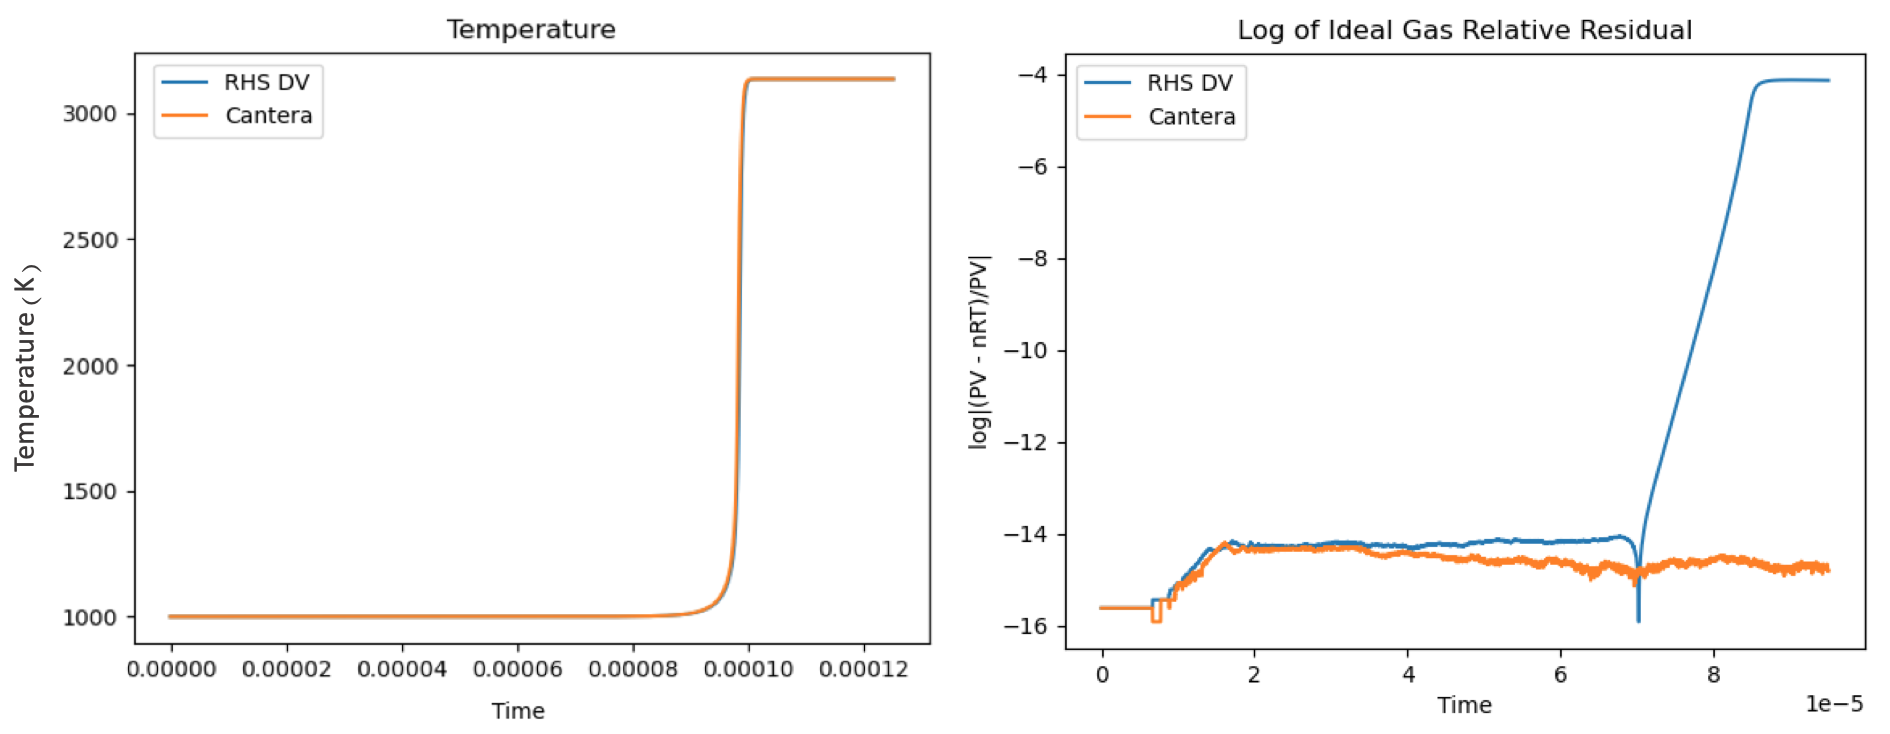
\includegraphics[width=0.8\linewidth,trim=4 4 4 4,clip]{figures/autoignition_drift.png}
	\caption{Temperature profiles (left) and relative ideal gas law residual (right)
		 for advancement of homogeneous H2-O2 autoignition example (employing the nine-species
		 San Diego mechanism \cite{sandiego}) using a fully differential approach (blue) versus a differential-algebraic
		 approach (orange) where the constant internal energy and ideal gas law constraints are fulfilled
		 by a Newton solve within Cantera \cite{cantera}.}
\label{fig:autoignition_drift}
\end{figure}
To avoid drift off of the ideal gas law manifold, a chemical
kinetic Jacobian modified to include the algebraic constraints explicitly can
be used. This approach, detailed in Hung \cite{hung2003algorithms}, modifies the molar source terms to incorporate
this constraint while removing the temperature and pressure source terms (which
we then replace with a temperature Newton solve based on the constant internal
energy constraint via Cantera \cite{cantera}, as well as a direct application of the ideal
gas law to obtain the pressure). This modified Jacobian can be expressed as
\begin{align}
J^{*} = \begin{bmatrix}	\frac{d\dot{n}_{1}^{*}}{dn_{1}} & \hdots & \frac{d\dot{n}_{1}^{*}}{dn_{N_{sp}-1}} \\
	                \vdots & \ddots & \vdots \\
	                \frac{d\dot{n}_{N_{sp}-1}^{*}}{dn_{1}} & \hdots & \frac{d\dot{n}_{N_{sp}-1}^{*}}{dn_{N_{sp}-1}}, \\
    \end{bmatrix}
\end{align}
where
\begin{align}
\frac{d\dot{n}_{i}^{*}}{dn_{j}} = \frac{d\dot{n}_{i}}{dn_{j}} - \frac{U_{j}}{C_{v}}\frac{d\dot{n}_{i}}{dT}.
\end{align}
In this expression, $U_{j}$ is the contribution of the $j$-th species to the
internal energy, and $C_{v}$ is the specific heat of the mixture at constant
volume.

Which of these Jacobians is ideal for our purposes is a consideration worth
monitoring as our implicit integration techniques develop. In particular, 
a third relatively unexplored approach would use the fully differential
method with pressure and temperature source terms, while also using penalization
to force the solution towards the constraint manifold. This attenuation approach
is described in some detail (albeit for smaller model problems) by Ascher and
Petzold \cite{ascher1998computer}.

\subsubsection{Timestep Control Algorithm}

%%%%% CANDIDATE FOR REMOVAL
%Early implicit-explicit runs of small-scale reacting flow problems
%quickly identified a need to adapt the timestep of the integrator based
%on relative and/or absolute local error demands. We therefore employ a
%timestep control algorithm which, in its current form, is that of ODE45 \cite{dormand1980family}, wherein
%a timestep multiplier $r$ is calculated based on a local error estimate constructed from
%state estimates of two (differing) explicit orders:
%\begin{align}
%r = \frac{\|s_{q+1} - s_{q}\|_{2}}{\text{ATOL} + \text{RTOL} \cdot \text{max}(\|s_{q}\|_{2}, \|s_{q+1}\|_{2})}
%\end{align}
%Here, $s_{q}$ is the state estimate obtained using an order-$q$ scheme, and ATOL and RTOL are absolute and
%relative error tolerances specified by the user. Once $r$ is calculated, the timestep is \emph{decreased} if
%$r>=1$ via
%\begin{align}
%\Delta t = 0.9\Delta t (r)^{-1/q}
%\end{align}
%and \emph{increased} if $r<1$ via
%\begin{align}
%\Delta t = 0.9\Delta t (r)^{-1/(q+1)}
%\end{align}

%Another form under consideration is that of CVODE, which makes use of a weighted
%root-mean-square norm to more adequately handle states with components that
%feature a large variation in magnitude. The weights are calculated as
%%%%% END CANDIDATE FOR REMOVAL
Early implicit-explicit runs of small-scale reacting flow problems
quickly identified a need to adapt the timestep of the integrator based
on relative and/or absolute local error demands. We therefore employ a
timestep control algorithm which, in its current form, is similar to that of CVODE,
using a weighted root-mean-square norm to more adequately handle states with
components that feature a large variation in magnitude. The weights are calculated as
\begin{align}
w_{i} = \frac{1}{\text{ATOL} + \text{RTOL} \lvert s_{q,i} \rvert}
\end{align}
with the weighted root-mean-square norm then being given by
\begin{align}
\|E\|_{wrms} = \left(\sum_{i=1}^{N} \frac{1}{N} (w_{i}(s_{q+1,i} - s_{q,i}))^2 \right)^{1/2},
\end{align}
where $s_{q,i}$ is the $i$-th component of the state estimate obtained using an order-$q$ scheme.
The timestep is \emph{decreased} if $\|E\|_{wrms} \geq 1$ via
\begin{align}
\Delta t = 0.9\Delta t (\|E\|_{wrms})^{-1/q}
\end{align}
and \emph{increased} if $\|E\|_{wrms}<1$ via
\begin{align}
\Delta t = 0.9\Delta t (\|E\|_{wrms})^{-1/(q+1)}.
\end{align}

%Regardless of the error norm used, this added capability alone presents a number of
This added capability presents a number of
questions in terms of how best to accomplish this error control. In particular,
step ratio adjustment \emph{in situ}, rather than timestep adjustment, to meet error
needs provides an implementation challenge in terms of code generation of these
integrators, whereas the choice of which solution component(s) are involved in error
estimation/timestep control also presents a design decision that could have notable
effect on numerical performance.

%===========================================================================
\subsection{Validation Plan}

The efficacy of the time integrators constructed via the above methodology will
be assessed using a reacting mixing layer problem with a hyperbolic tangent velocity profile
for the baseflow (as used by \cite{michalke1964inviscid} and \cite{blumen1970shear}), with
the San Diego 9-species chemical mechanism \cite{sandiego} employed for the chemical kinetics. By perturbing
this baseflow with the mode having the highest growth rate to instability (reproduced based
on the inviscid analyses of \cite{michalke1964inviscid} and \cite{blumen1970shear}), and by
varying the temperature in the domain to induce ignition local to the mixing layer, we can
establish a fast-evolving solution component (the chemical kinetics of the ignition) and a
slow-evolving solution component (the fluid motion), both possessing accessible
means of rate modification (for the chemistry, we can accomplish this by scaling the
pre-exponential factors in the Arrhenius reaction rates, and for the fluid, we can scale
the magnitude of the initial crossflow velocity).
\begin{figure}
\centering
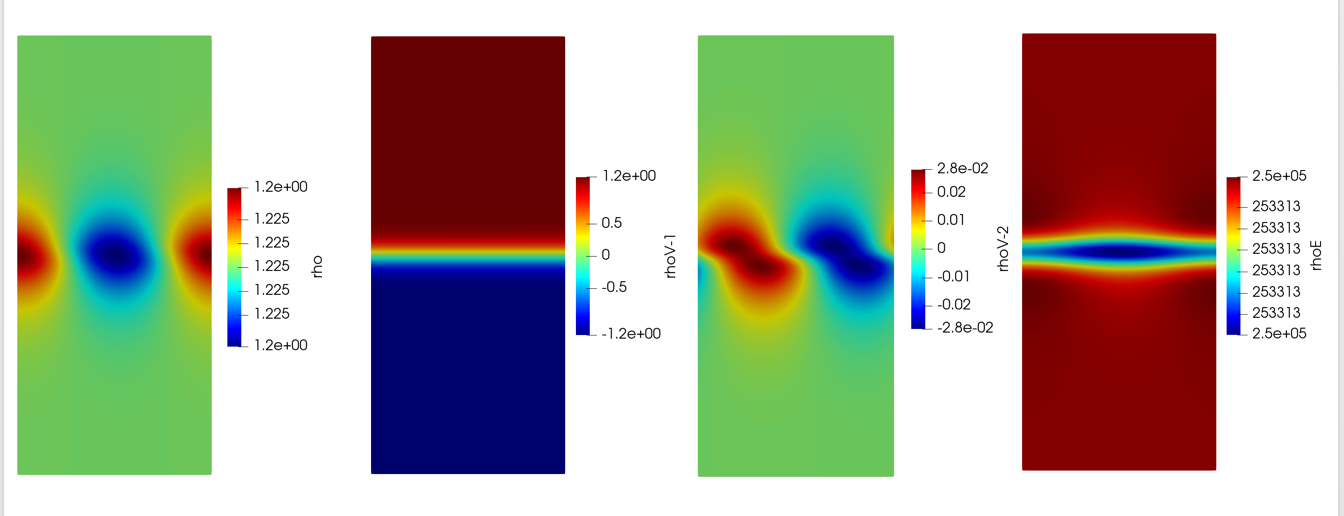
\includegraphics[width=0.9\linewidth,trim=4 4 4 4,clip]{figures/hyperbolic_tangent_air.png}
\caption{Perturbed initial condition of the hyperbolic tangent example - sea-level air.}
\label{fig:hyperbolic_cold_rhov2}
\end{figure}
In doing so, what should result is a problem with ample testbed capabilities for our
new multi-rate integrators, and also a problem firmly rooted in physical utility in that
it provides the simplest model for scramjet/ramjet combustion processes.

%===========================================================================
\subsection{Outlook}

\subsubsection{Current Status}

At present, implicit-explicit time integration of reacting flows using Runge-Kutta
based methods in conjunction with code generation of source terms and Jacobians for
the chemical mechanisms is implemented and undergoing testing with the fluid solver
application. Implicit Adams methods (with single-rate Adams-Moulton being the baseline)
for the purposes of chemistry integration are also being implemented, along with
an application of the error-informed timestep control algorithm to both
single-rate and multi-rate Adams methods. Construction of implicit-explicit multi-rate
Adams methods with error-informed adaptivity are well underway, with testing
of fully-explicit adaptive Adams multi-rate integrators on a stiff small-scale Cantera
\cite{cantera} two-reactor system in progress. A schematic of this problem, which is
based in large part on an example problem bundled with the software, is given in
Figure \ref{fig:cantera_reactors}.
\begin{figure}
\centering
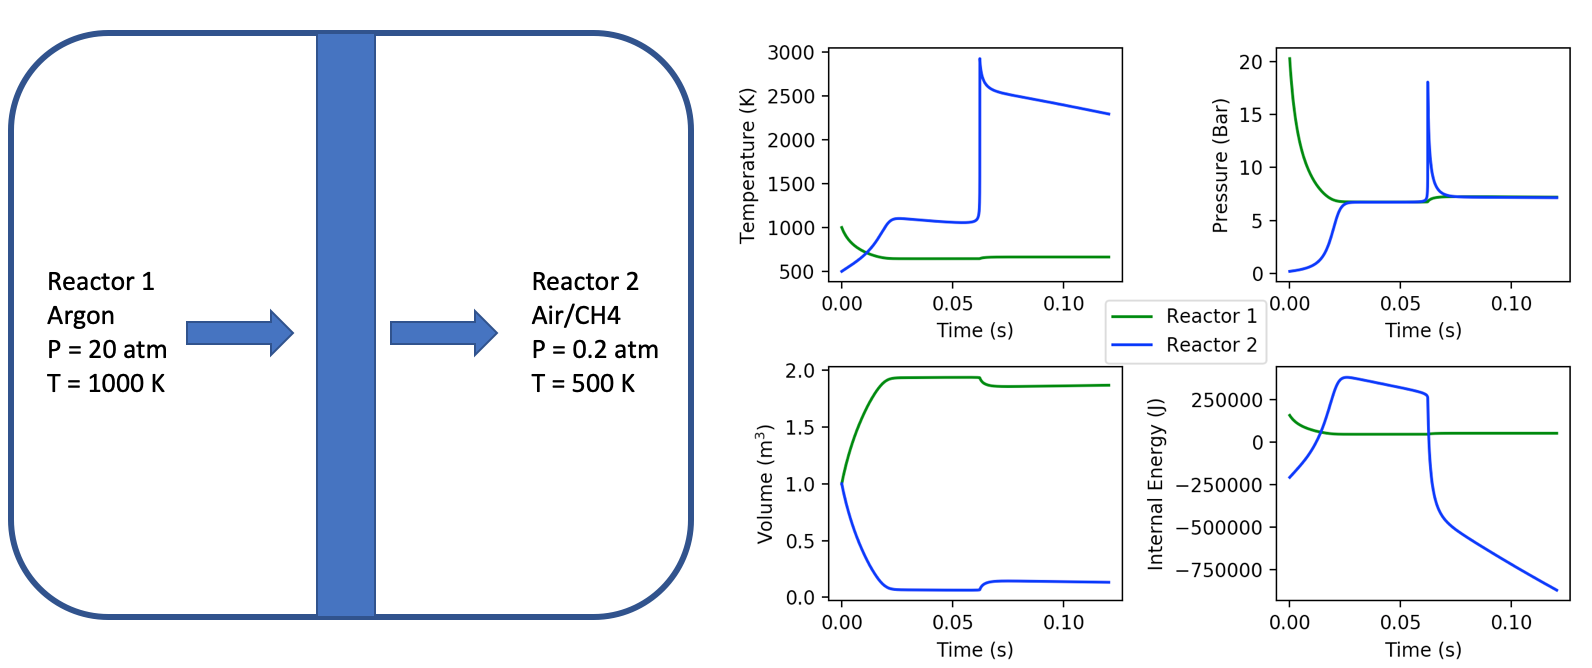
\includegraphics[width=0.9\linewidth,trim=4 4 4 4,clip]{figures/cantera_reactors_soln.png}
\caption{Cantera two-reactor example problem. The solution shown is obtained using
	 Cantera's internal reactor system integrator, which is based on the same
	 BDF algorithm employed by CVODE. The piston velocity is initially zero,
	 with ignition eventually occuring in the air-methane reactor.}
\label{fig:cantera_reactors}
\end{figure}
While the governing equations for this problem are not the same as those generated
by PyJac-V2, our hope is that it will serve as a suitably small stiff test problem to be
used as a stepping stone in verification of the error-informed timestep controller
for explicit methods, as well as further exploration of its efficacy.

As for the reacting crossflow validation problem, an initial setup employing
cold flow (no autoignition) with the perturbed baseflow applied to sea level air
is complete (see Figure \ref{fig:hyperbolic_cold_rhov2}), with validation via the
growth rate of the unstable mode completed. Also implemented in the reacting flow
solver is a one-dimensional laminar free flame problem, which may also be used
as a first-pass validation (via comparison to the Cantera-estimated steady-state
flame speed) for new integration methods for reacting flows as they become available.
A basic description of this case, as well as flame speed data generated via a Leap-generated
IMEX ARK integrator using PyJac-V2 analytical Jacobians, is given in the next section.

\subsubsection{Risk Mitigation}

Assuming demonstration of improved
performance and/or accuracy of the \emph{multi-rate} integrators over the
state-of-the-art is for reasons unforseen impossible, a "fallback" takeaway
would be demonstration of improvement over a low-order splitting
approach via Leap implementation of an existing IMEX Runge-Kutta based scheme
\cite{kennedy2003additive} that treats the chemistry implicitly via code-generated
analytical Jacobians. Given the use of a coupled implicit-explicit scheme
(for which high order has already been proven in other circumstances),
as well as a chemical Jacobian that is more accurately and efficiently obtained
than via finite differences (the method of CVODE), this outcome should be attainable
at minimum.

As a step towards proving this, we have implemented a small-scale one-dimensional
free-flame test, wherein we use a code-generated implementation of the fourth-order
additive Runge-Kutta scheme of Kennedy and Carpenter to drive a simulation of
a premixed, freely propagating hydrogen flame with an unburned gas temperature
of 300 K at a pressure of one atmosphere (see Figure \ref{fig:freeflame_output}). Comparing the estimated laminar
flame speed to that of a steady-state analysis performed by Cantera at a number
of equivalence ratios $\phi$, we see suitable agreement of less than 3\% error, indicating
that the reacting flow equations - and in particular the chemical source terms and Jacobians -
are correctly implemented and ready for both further experimentation with multi-rate
timescale splitting and a more thorough analysis of performance.
\begin{figure}
\centering
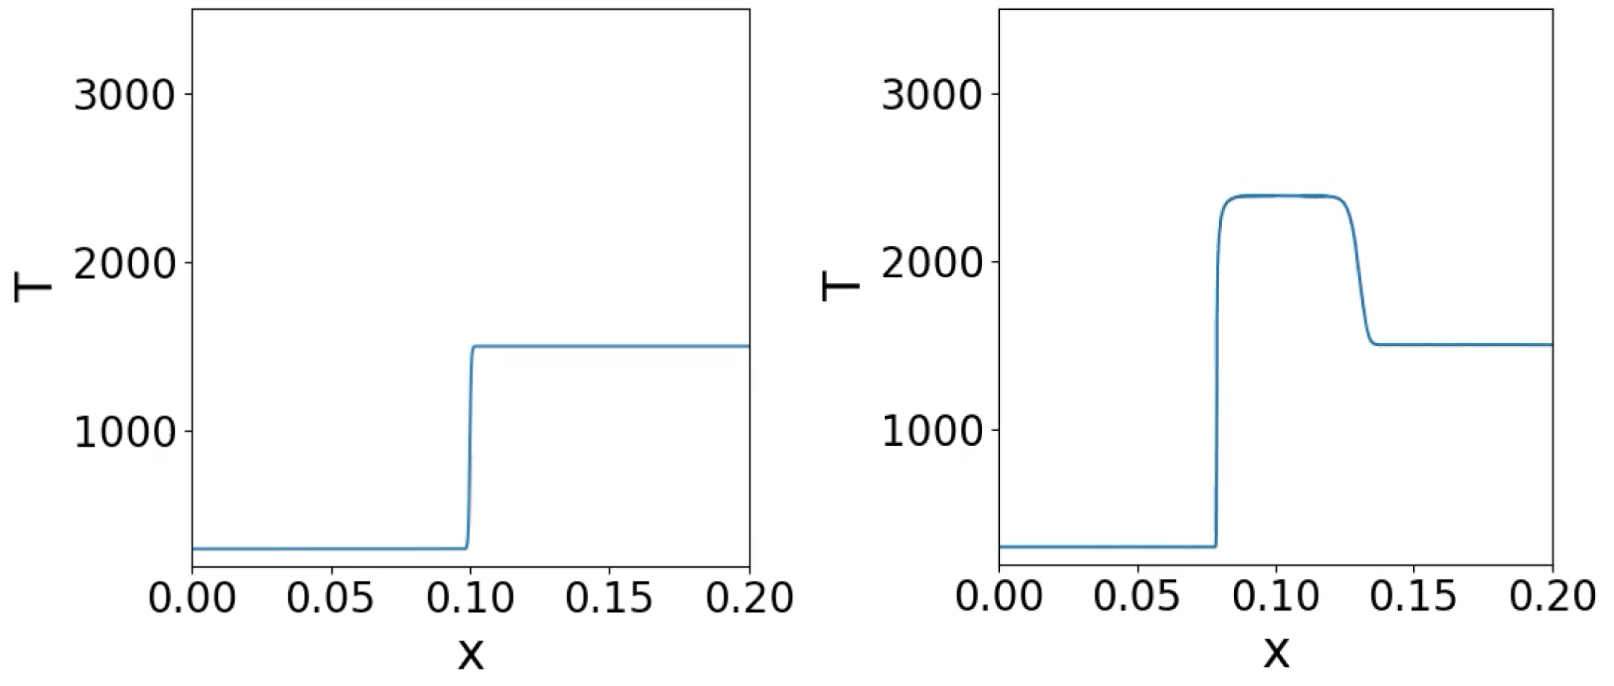
\includegraphics[width=0.9\linewidth,trim=4 4 4 4,clip]{figures/flame_figures.png}
\caption{Figures showing the temperature profile of the one-dimensional free-flame example
         at initial condition (left) and after 0.0025 seconds (right).}
\label{fig:freeflame_output}
\end{figure}

{
\centering
\begin{tabular}{cccc}\hline
$\phi$ & Leap $S_{L}$ (m/s) & Cantera $S_{L}$ (m/s) & \% Error \\ \hline
0.75 & 1.585566 & 1.599170 & 0.85 \\
1.0 & 2.351950 & 2.421837 & 2.89 \\
1.5 & 3.1734067 & 3.153888 & 0.62 \\ \hline
\end{tabular}
\captionof{table}{Comparing the laminar flame speeds estimated by Leap-PyJac-V2
	          chemistry integration and by Cantera's steady-state analysis.}
}

%===========================================================================
